%%% Econ711: Microeconomics I
%%% Fall 2020
%%% Danny Edgel
%%%
% Optional, but due on Canvas Monday, December 14, 11:59pm Central Time
%%%

%%%
%							PREAMBLE
%%%

\documentclass{article}

%%% declare packages
\usepackage{amsmath}
\usepackage{amssymb}
\usepackage{array}
\usepackage{bm}
\usepackage{changepage}
\usepackage{centernot}
\usepackage{graphicx}
\usepackage{multirow}
\usepackage[shortlabels]{enumitem}
\usepackage{fancyhdr}
	\fancyhf{} % sets both header and footer to nothing
	\renewcommand{\headrulewidth}{0pt}
    \rfoot{Edgel, \thepage}
    \pagestyle{fancy}
	
%%% define shortcuts for set notation
\newcommand{\N}{\mathbb{N}}
\newcommand{\Z}{\mathbb{Z}}
\newcommand{\R}{\mathbb{R}}
\newcommand{\Q}{\mathbb{Q}}
\newcommand{\lmt}{\underset{x\rightarrow\infty}{\text{lim }}}
\newcommand{\neglmt}{\underset{x\rightarrow-\infty}{\text{lim }}}
\newcommand{\zerolmt}{\underset{x\rightarrow 0}{\text{lim }}}
\newcommand{\usmax}[1]{\underset{#1}{\text{max }}}
\newcommand{\usmin}[1]{\underset{#1}{\text{min }}}
\newcommand{\intersect}{\bigcap}
\newcommand{\union}{\bigcup}
\newcommand{\olw}{\overline{w}}
\newcommand{\olx}{\overline{x}}
\newcommand{\loge}[1]{\text{log}\left(#1\right)}
\renewcommand{\P}{\mathcal{P}}
\renewcommand{\L}{\mathcal{L}}
\newcommand{\olp}{\overline{p}}
\renewcommand{\exp}[1]{\text{exp}\left\{#1\right\}}
\newcommand{\binv}[1]{b_j^{-1}\left(#1\right)}

\DeclareMathOperator{\E}{\mathbb{E}}% expected value

%%% define column vector command (from Michael Nattinger)
\newcount\colveccount
\newcommand*\colvec[1]{
        \global\colveccount#1
        \begin{pmatrix}
        \colvecnext
}
\def\colvecnext#1{
        #1
        \global\advance\colveccount-1
        \ifnum\colveccount>0
                \\
                \expandafter\colvecnext
        \else
                \end{pmatrix}
        \fi
}

%%% define function for drawing matrix augmentation lines
\newcommand\aug{\fboxsep=-\fboxrule\!\!\!\fbox{\strut}\!\!\!}

\makeatletter
\let\amsmath@bigm\bigm

\renewcommand{\bigm}[1]{%
  \ifcsname fenced@\string#1\endcsname
    \expandafter\@firstoftwo
  \else
    \expandafter\@secondoftwo
  \fi
  {\expandafter\amsmath@bigm\csname fenced@\string#1\endcsname}%
  {\amsmath@bigm#1}%
}


%________________________________________________________________%

\begin{document}

\title{	Homework \#6 }
\author{ 	Danny Edgel 					\\ 
			Econ 711: Microeconomics I		\\
			Fall 2020						\\
		}
\maketitle\thispagestyle{empty}

\noindent\textit{Collaborated with Sarah Bass, Emily Case, Michael Nattinger, and Alex Von Hafften}

%%%________________________________________________________________%%%

\subsection*{Question 1}
In order for ${\left\{(C,C),(C,C),...\right\}}$ to be supported in a subgame perfect equilibrium, it must be the case that neither player has incentive to deviate and earn a one-time payoff of 8 despite getting a lower payoff of 1 in each period thereafter. Thus, in each period, the following condition must be satisfied:
\[
	\sum_{t=0}^\infty 2\delta^t \geq 8 + \sum_{t=1}^\infty \delta^t
\]
Solving this for $\delta$ yields:
\begin{align*}
	2\left(\frac{\delta}{1-\delta}\right) &\geq 8 + \frac{\delta}{1-\delta}	\\
	\delta &\geq 6(1-\delta)	\\
	\delta &\geq \frac{6}{7}
\end{align*}	
Thus, ${\delta\in\left[\frac{6}{7}\right]}$ in order for ${\left\{(C,C),(C,C),...\right\}}$ to be supported in a subgame perfect equilibrium.


%%%________________________________________________________________%%%

\subsection*{Question 2}

\begin{enumerate}[(a)]
	\item In order for ${(\sigma_1,\sigma_2)}$ to be an SPE, it must the case that a one-time deviation to $D$, which earns a payoff of 3, is outweighed by a one-time penalty of 0. this is true when the following inequality is satisfied:
		\[
			2 + 2\delta + \sum_{t=2}^\infty 2\delta^t \geq 3 + 0\delta + \sum_{t=2}^\infty 2\delta^t
		\]
		Solving for $\delta$,
		\begin{align*}
			2 + 2\delta &\geq 3	\\
			\delta &\geq \frac{1}{2}
		\end{align*}	
	
	\item If $(P,P)$ resulted in a payoff of $1/2$ for both players, then the condition would become:
		\begin{align*}
			2 + 2\delta &\geq 3	 + \frac{1}{2}\delta\\
			\delta &\geq \frac{2}{3}
		\end{align*}	
	
	\item As I explained in (a), the condition for sustaining ${(\sigma_1,\sigma_2)}$ as an SPE is ensuring that the penalty of deviation to $(P,P)$ is large enough keep it in your opponent's best interest from deviating to their higher-payoff outcome (of $(C,D)$ or $(D,C)$). Increasing the payoff from the penalty outcome requires a higher weight on the difference between the equilibrium-path outcome (2) relative to the penalty outcome (1/2). Since the penalty outcome occurs in the period after the hypothetical deviation, a lower $\delta$ decreases the penalty from deviation.
	
	\item Presuming that the question is ``for what set of $(P,P)$ payoffs does their exist a ${\delta<1}$ such that ${(\sigma_1,\sigma_2)}$ can be supported as an SPE?", we must determine the symmetric payoff, $x$, that satisfies:
		\[
			\underset{\delta\rightarrow 1^-}{\text{lim }}\left\{2 + 2\delta\right\} \geq \underset{\delta\rightarrow 1^-}{\text{lim }}\left\{3	 + x\delta\right\} 
		\]
		To understand what this means for all feasible values of $x$ given some ${\delta<1}$, we can solve for x and relate that solution to ${\delta=1}$:
		\[
			x \leq 2 - \frac{1}{\delta} < 1
		\]
		Thus, in order for ${(\sigma_1,\sigma_2)}$ to be supported as an SPE, the symmetric payoff from $(P,P)$ must be less than 1.
	
\end{enumerate}

%%%________________________________________________________________%%%

\subsection*{Question 3}

\begin{enumerate}[(a)]
	\item On this equilibrium path, the player with an incentive to deviate is the $C$ player, who prefers a payoff of 0 to a payoff of -1. Since any player can trigger the 0 payoff, this requires no coordination and can thus be used as a punishment, since the deviating player would have otherwise received a payoff of 2 during the punishment round. The pure strategy profile for this equilibrium, then, is:
		\begin{enumerate}[(I)]
			\item Play $(A,B,C)$ initially, or if $(C,A,B)$ was played last. Play $(B,C,A)$ if $(A,B,C)$ was played last and $(C,A,B)$ if $(B,C,A)$ was played last
			\item If there is a deviation from (I), play $(D,D,D)$ (or any other play that involves a non-deviating player playing $D$) once, then restart (I)
			\item If there is a deviation from (II), then restart (II)
		\end{enumerate}
		An equilibrium path with this pure strategy profile can be supported if the payoff from the equilibrium path at least matches that of a deviation from it:
		\begin{align*}
			-1 + 2\delta + 0\delta^2  &\geq 0 + 0\delta + 0\delta^2	\\
			\delta &\geq \frac{1}{2}
		\end{align*}
		Thus, this strategy profile is an SPE if ${\delta\geq\frac{1}{2}}$.
	
	\item In this new equilibrium, the deviating player is slated (under the equilibrium path) to play $B$ following their deviation, rather than $A$. Under the old punishment scheme, each player would prefer deviating to the equilibrium path under any $\delta$. An alternative is to adopt a new punishment scheme that deviates to $(D,D,D)$ for some $L$ periods where the deviating player was slated to play $A$. Under any of these equilibrium plays that could sustain the new path, the old path could also be sustained in the old equilibrium with an even lower $\delta$. This is because, under any $\delta$, it takes a lower $\delta$ to punish a deviation when the player with an incentive to deviate would get their maximum payoff (of 2, in this case) immediately following their deviation were they not to deviate.
	
\end{enumerate}


%%%________________________________________________________________%%%

\subsection*{Question 4}

\begin{enumerate}[(a)]
	\item An equivalent behavioral strategy is presented below.
		\[
			\beta_1 = \left(\left(\beta_1(A),\beta_1(B)\right),\left(\beta_1(E),\beta_1(F),\beta_1(G)\right)\right) = \left(\left(\frac{5}{6},\frac{1}{6}\right),\left(0,\frac{1}{2},\frac{1}{2}\right)\right)
		\]
	
	\item Each of the mixed strategies involving A must be played with frequencies that sums to $\frac{1}{3}$. In other words,
		\[
			\sigma_1(AE) + \sigma_1(AF) + \sigma_1(AG) = \beta_1(A) = \frac{1}{3}
		\]
		Half of the time that $B$ is played, $E$ is also played. The other half of the time is split between $F$ and $G$. Since $B$ is played $\frac{2}{3}$ of the time,
		\[
			\sigma_1(BE) = \frac{1}{3}\text{, }\sigma_1(BF)=\sigma_1(BG)=\frac{1}{6}
		\]
	
\end{enumerate}


	


%%%________________________________________________________________%%%

\subsection*{Question 5}
To compute the sequential equilibria of this game, let us consider possible beliefs held by player 3, then deduce consistent and sequentially rational strategies by each player:
\begin{enumerate}
	\item $\mu(D) = \mu(d) = 0$
		\begin{align*}
			\text{sequential rationality} 	&\Rightarrow \text{ player 3's information set is never reached, so }\beta_3(R)\in[0,1] \\
			\text{sequential rationality} 	&\Rightarrow \beta_2(d) = 0	\text{ if }\beta_3(R)\in\left[0,\frac{2}{3}\right)\\
			\text{sequential rationality} 	&\Rightarrow \beta_1(D) = 0 \text{ if }\beta_2(a)\geq\frac{1}{2}\beta_3(R)	\\
			\text{consistency}				&\Rightarrow \mu(D) = \mu(d) = 0	
		\end{align*}
		$\therefore$ ${\mu(D) = \mu(d) = 0}$, ${\beta_1(D)=0}$, ${\beta_2(d)=0}$, and ${\beta_3(R)\in[0,\frac{2}{3})}$ is a sequential equilibrium 
		
	\item $\mu(D) = \mu(d) = 1$
		\begin{align*}
			\text{sequential rationality} 	&\Rightarrow \beta_3(L) = 1	\\
			\text{sequential rationality} 	&\Rightarrow \beta_2(d) = 0	\\
			\text{sequential rationality} 	&\Rightarrow \beta_1(D) = 0	
		\end{align*}
		$\mu$ is not consistent, so $(\beta,\mu)$ is not a sequential equilibrium
		
	\item $\mu(D)\in(0,1)\land \mu(d) = 1$
		\begin{align*}
			\text{sequential rationality} 	&\Rightarrow \beta_3(L) = 1	\\
			\text{sequential rationality} 	&\Rightarrow \beta_2(d) = 0	\\
			\text{sequential rationality} 	&\Rightarrow \beta_1(D) = 0	
		\end{align*}
		$\mu$ is not consistent, so $(\beta,\mu)$ is not a sequential equilibrium
		
	\item $\mu(D) = 1\land \mu(d)\in(0,1)$
		\begin{align*}
			\text{sequential rationality} 	&\Rightarrow \beta_3(L) = 1	\\
			\text{sequential rationality} 	&\Rightarrow \beta_2(d) = 0	\\
			\text{sequential rationality} 	&\Rightarrow \beta_1(D) = 0	
		\end{align*}
		$\mu$ is not consistent, so $(\beta,\mu)$ is not a sequential equilibrium
		
	\item $\mu(D)\in(0,1)\land \mu(d)\in(0,1)$
		\begin{align*}
			\text{sequential rationality} 	&\Rightarrow \beta_3(R)\in(0,1) \text{ if } \frac{\beta_1(D)}{\beta_1(D) + (1-\beta_1(D))\beta_2(d)}= \frac{2}{3}\\
			\text{sequential rationality} 	&\Rightarrow \beta_2(d)\in(0,1)	\text{ if } \beta_3(R)=\frac{2}{3} \\
			\text{sequential rationality} 	&\Rightarrow \beta_1(D)\in(0,1)	\text{ if } \frac{\beta_2(a)}{\beta_3(R)}=\frac{1}{2}	
		\end{align*}
		$\therefore$ there is a mixed-strategy equilibrium at:
		\[
			\left\{\left(\mu(D),\mu(d)\right),\left(\beta_1(D),\beta_2(d),\beta_3(R)\right)\right\} 
				= \left\{\left(\frac{1}{3},\frac{1}{4}\right),\left(\frac{4}{7},\frac{1}{4},\frac{2}{3}\right)\right\}
		\]
\end{enumerate}





%%%________________________________________________________________%%%

\subsection*{Question 6}


	


%%%________________________________________________________________%%%

\subsection*{Question 7}
Let $x$ be the top node for player 2 and $\mu(x)$ be player 2's belief that she is at the top node. Regardless of which node player 2 is on, $B$ is dominated by one of the other two moves, so ${\beta_2(T) + \beta_2(M) = 1}$. \\
\\
After removing $B$ from play, $I$ is dominated by $O$ for player one if player 1 is of type $t_b$. Thus, in order for beliefs to be consistent, ${\mu(x) = 1}$. Sequential rationality then dictates that ${\beta_2(T)=1}$. Given $\beta_2$, player 1's sequentially rational move when type $t_a$ is $I$. Thus, there is a separating sequential equilibrium at
\[
	\{\left\{(\beta_{t_a}(I),\beta_{t_b}(I),\beta_2(T)),\mu(x)\right\} = \{\left\{(1,0,1),1\right\}
\]
In order for the intuitive criterion to be violated, one of player 1's types would have have a strictly dominant strategy that would enable them to make a higher payoff than the equilibrium payoff were they to deviate to it. The only possible payoff improvement for player 1 is if $t_b$ could play $I$ and have player 2 play $B$. However, following ISD, $I$ is strictly dominated for $t_b$. Thus, the intuitive criterion is not violated. \\
\\
Suppose that ${\mu(x)\leq0.5}$. Then, player 2's sequentially rational strategy is to play ${\beta_2(M)=0}$ if ${\mu(x)<\frac{1}{2}}$ and to mix with ${\beta_2(T)\leq\frac{1}{3}}$ if ${\mu(x)\leq0.5}$. This is a pooling equilibrium where both types of player 1 choose to play $O$ and player 2 is never driven to update her beliefs about the behavior of player 1. However, were player 1 to deviate, player 2 would recognize that such a deviation is dominated by $O$ for type $t_b$. Thus, a best response for player 2 would be to play ${\beta_2(T)=1}$. Therefore, this equilibrium does not satisfy the intuitive criterion.

	


%%%________________________________________________________________%%%

\subsection*{Question 8}

\begin{enumerate}[(a)]
	\item An extensive form game, $\Gamma$, of this interaction is drawn below.
		\begin{center}
			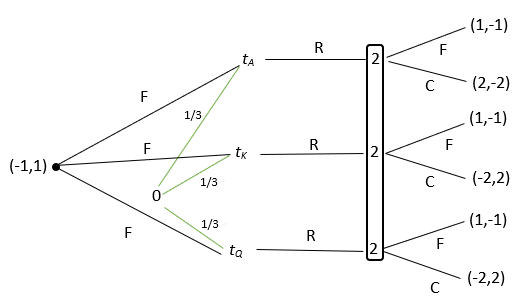
\includegraphics[scale=.8]{figure8a.png}
		\end{center}
	
	\item Player 1 could be of three possible types, under each of which she can have a different strategy. Thus,
	\[
		S_1 = \left\{RRR,RRF,RFF,FFF,FFR,FRR,FRF,RFR\right\}\text{, }S_2 = \left\{C,F\right\}
	\]
	
	\item As far as either player is concerned, player 1 drawing a queen is identical to player 1 drawing a king. $F$ is strictly dominated for $t_A$, so there is no equilibrium in which ${\beta_{t_A}(F)>0}$. If player 2 plays a pure strategy of always folding (say, because ${\mu(t_A)=1}$), then player 1 will have an incentive to raise regardless of what card she draws. 
	
	This cannot be an equilibrium, because any beliefs with which this pure strategy from player 2 are rational would then not be consistent. On the other hand, the pure strategy ${\beta_2(C)=1}$ is sequentially rational if ${\mu(t_A)\leq \frac{3}{4}}$. Player 1's only sequentially rational response to this strategy is to only raise if she draws an ace, rendering $\mu$ inconsistent. Thus, there are no equilibria in which player 2 plays a pure strategy.

	Player 2 is willing to mix if ${\mu(t_A) = \frac{3}{4}}$, and these beliefs are only consistent in a pooling equilibrium. According to Bayes rule,
		\[
			\mu(t_A) = \frac{\frac{1}{3}\beta_{t_A}(R)}{\frac{1}{3}\left(\beta_{t_A}(R)+\beta_{t_K}(R)+\beta_{t_Q}(R)\right)}
				= \frac{1}{1+\beta_{t_K}(R)+\beta_{t_Q}(R)}
		\]
	Then, in order for beliefs to be consistent, ${\beta_{t_K}(R)+\beta_{t_Q}(R)=\frac{1}{3}}$. In order for player 1 to mix with these weights when she doesn't draw an ace, she must be indifferent between raising and folding, based on player 2's strategy:
		\[
			-2\beta_2(C)+1-\beta_2(c) = -1 \iff \beta_2(C) = \frac{2}{3}
		\]
	Therefore, there appears to be one sequential equilbrium at:
		\[
			\left\{\left(\left(\beta_{t_A}(R),\beta_{t_K}(R),\beta_{t_Q}(R)\right),\beta_2(C)\right),\mu(t_A)\right\} = \left\{\left(\left(1,\left[0,\frac{1}{3}\right],\frac{1}{3}-\beta_{t_K}(R)\right),\frac{2}{3}\right),\frac{3}{4}\right\}
		\]
\end{enumerate}

%%%________________________________________________________________%%%


\end{document}






To compute the sequential equilibria of this game, let us walk through each possible weight player 3 places on $R$, then consider which moves by other players would be sequentially rational to determine whether the move is an equilibrium.
\begin{enumerate}
	\item $\beta_3(R)\in[0,\frac{2}{3})$
		\begin{align*}
			\text{sequential rationality} 	&\Rightarrow \beta_2(d) = 0	\\
			\text{sequential rationality} 	&\Rightarrow \beta_1(D) = 0	\\
			\text{consistency}				&\Rightarrow \mu(D) = \mu(d) = 0	\\
			\text{sequential rationality} 	&\Rightarrow \beta_3(R)\in(0,\frac{2}{3}) \text{ (player 3's information set is never reached)}
		\end{align*}
		$\therefore$ $(\beta,\mu)$ \textbf{is} a sequential equilibrium 
		
	\item $\beta_3(R)\in[\frac{2}{3},1]$
		\begin{align*}
			\text{sequential rationality} 	&\Rightarrow \beta_2(d) = 1	\\
			\text{sequential rationality} 	&\Rightarrow \beta_1(D) = 1	\\
			\text{consistency}				&\Rightarrow \mu(D) = 1		\\
			\text{sequential rationality} 	&\Rightarrow \beta_3(R) = 0
		\end{align*}
		$\therefore$ $(\beta,\mu)$ is not a sequential equilibrium
\end{enumerate}




	To find a sequential equilibrium, let us consider each possible set of beliefs for player 2:
		\begin{enumerate}
			\item $\mu(t_A) = 1$
				\begin{align*}
					\text{sequential rationality} 	&\Rightarrow \beta_2(F) = 1	\\
					\text{sequential rationality} 	&\Rightarrow \beta_{t_k}(C) = \beta_{t_Q}(C) = 1 \\
					\text{consistency} 				&\Rightarrow \mu(t_A) < 1	
				\end{align*}
				Under this belief, player 1 has an incentive to call regardless of what she draws, so $\mu$ is not consistent and cannot be part of a sequential equilibrium. 
				
			\item $\mu(t_A) = 0$
				\begin{align*}
					\text{sequential rationality} 	&\Rightarrow \beta_2(F) = 0							\\
					\text{sequential rationality} 	&\Rightarrow \beta_{t_k}(C) = \beta_{t_Q}(C) = 0 	\\
					\text{sequential rationality} 	&\Rightarrow \beta_{t_A}(C) = 1 					\\
					\text{consistency} 				&\Rightarrow \mu(t_A) > 0	
				\end{align*}
				This belief ignores the dominance of calling whenever player 1 draws an ace, so $\mu$ is not consistent and cannot be part of a sequential equilibrium. 

		\end{enumerate}























